
\documentclass[11pt]{article} % Font size
\usepackage[a4paper, total={6in, 10.5in}]{geometry} % Margins

\usepackage{graphicx}
\usepackage[simplified]{pgf-umlcd}
\usepackage{tikz}


\title{\textbf{CSCI 447 - Project 1}}
\author{Wilson Harris | Matthew Nitschke | Alex Abrahamson }
\date{September 11, 2017}

\begin{document}
\maketitle

\section{Description of the Problem}
The problem is simply the conversion of data from the UCI ML repository (which is in CSV format) to ARFF format, which is the format required by WEKA. This involves having the software find out how many attributes are in the CSV file, what the attributes are/can be, and how to rearrange each individual line to fit the ARFF format. The largest problem for the utility is to determine the datatype of each attribute that is listed in the first row of the CSV file. While the first row (in a CSV file) lists the name of each attribute, it does not list the datatype. The utility must look at each column of each row, and determine the datatype from there. This is done through command-line arguments, where the user enters the types when invoking the utility. If the utility receives its command-line arguments properly and the CSV file is properly formatted, then the end result is a well-formed ARFF file that has lost no data in the translation.

\section{ARFF Converter}

\subsection{Design}
Our ARFF converter is a simple cli application written in javascript and run via the javascript runtime environment Node.js. The parameters of the program ask for the filename of the .cvs file, and a list of attribute types. Once run, the program parses out the filename and attribute types. It then loops through each attribute type looking for types of "enum" or "date", where if encountered asks the user for enum properties or date format. After the arguments have been parsed, arffConvert reads the desired .csv file and extracts the header line. This line is split into an array by its commas and looped through appending its name and correlating attribute type at each iteration. Finally, the data of the csv file is processed by splitting each line into an array. Each column is formatted by encoding any invalid characters, and ensuring that if the columns type is a string, that the data is wrapped in quotes. After the data processing is complete the file is written to the user's current directory.

When designing this application the first decision to be made was to figure out how to get the attributes data types. We went through two iterations of this design, one used type inference by looking at the actual data of the csv file trying to guess what data type the column was, and the other simply required the user to enter each type as an argument when the program was called. We decided on the second option due to the lack of consistency in the csv files which caused for faulty type inference. Another problem which had to be fixed was dealing with commas within quotes. Csv files usually denote a string with a comma in it by surrounding the string with quotes. This breaks splitting each column by commas because the algorithm only looked for singular commas. A simple regex selector, found on stackoverflow, which ignores commas inside quotes was used to fix this problem. Finally, WEKA requires all strings to be wrapped in quotes. A simple format column function solved this problem by adding quotes to lines which needed them. Unfortunately a small problem surfaced when this was implemented. Because single quotes were used to wrap the data, any text with a single quote in it (such as i'm, that's, it's) broke the quote and henceforth broke the parse. To solve this, a find and replace is done on the data replacing any single quotes with their escaped counterpart: \textbackslash'.

\subsection{UML}
\begin{center}
  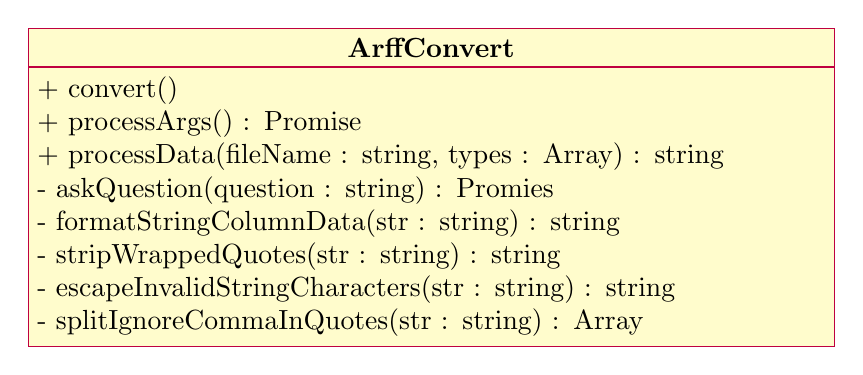
\begin{tikzpicture}
    \begin{class}[text width=10cm ]{ArffConvert}{0, 0}
      \operation{+ convert()}
      \operation{+ processArgs() : Promise}
      \operation{+ processData(fileName : string, types : Array) : string}
      \operation{- askQuestion(question : string) : Promies}
      \operation{- formatStringColumnData(str : string) : string}
      \operation{- stripWrappedQuotes(str : string) : string}
      \operation{- escapeInvalidStringCharacters(str : string) : string}
      \operation{- splitIgnoreCommaInQuotes(str : string) : Array}
    \end{class}
  \end{tikzpicture}
\end{center}

\subsubsection{convert()}
Convert is the function main call. It connects methods together, reads the .csv file, formats and then creates the new .arff file.

\subsubsection{processArgs()}
processArgs parses each command line argument passed in. It first extracts the fileName argument from the argsArray, and then proceeds to loop through each of the type arguments checking to see if they are date or enum types. If the type is date or enum the processArgs function asks the user what format or enum options to set that type to be. This function returns a promise to handle the asynchronous call that is used to get the users input.

\subsubsection{processData()}
The processData function call ensures that the data of the arff file is in the correct format. It loops through every line of the .csv file wrapping strings in quotes, and replaces invalid characters. It then returns a string of the formatted file.

\subsubsection{Utility Functions}
There are five private utility functions. Four of them are used to format strings, and the fifth is a simple function to wrap the Node.js readline call.

\section{Experimental Data}

\subsection{Data Sets}
We will use five different data sets.  When deciding what data sets to use, we considered two characteristics, the number of instances and attributes.  We expect these characteristics to be useful in detecting which algorithms take the longest to process data with different types of data sets.  We classified a low number of instances to be less than 500 and a high number to be greater than 1,000,000.  Attributes were classified as a low if less than 50 and high if greater than 100,000.  All of our data was retrieved from the UC Irvine Machine Learning Repository.  The first data set, Pems-SF, had a low number of instances and a high number of attributes.  The data described the occupancy of car lanes on the freeways in San Francisco.  Hemp mass, our second data set, had a high number of instances and a low number of attributes.  The data was produced by simulations of collisions that produce specific particles and their decay products. Next, we used a Parkinson Disease spiral drawing data set which had a low number or instances and attributes.  Subjects, some with Parkinson Disease, had their handwriting tested to see if Parkinson Disease can be identified through handwriting.  Our fourth data set had a high number of instances and attributes.  It is a set of URLs and their attributes with the goal of classifying malicious websites.  The final data set is a smartphone-based recognition of human activities data set.  It had a moderate number of instances and attributes.

\subsection{Machine Learning Algorithms}
We will be testing five learning algorithms:
\begin{enumerate}
	\item K-nearest neighbor
	\item Na\"{i}ve Bayes
	\item Logistic regression
	\item Decision tree with pruning
	\item Support vector machine with a nonlinear kernel
\end{enumerate}
These algorithms are already written on Weka, so the only editing of the algorithms will be tuning.

\subsection{Evaluation Measures}
We will evaluate the algorithms using two Weka analysis methods: Percent correct and elapsed time training.  Accuracy and speed are two common evaluations of machine learning algorithms.  (I need to try and find an article that can support this claim).  Percent correct is a useful evaluation for understanding the overall accuracy of an algorithm with a single number.  We chose elapsed time training because in our tests there will be more training data than testing data.  Therefore, the difference between times will likely be more significant.  K-nearest neighbor is an exception, because it is a lazy algorithm, but elapsed time training will provide valuable information on computation time for the other algorithms.

\section{References}
\end{document}
